\chapter{HPC projects on Twitter} \label{HPC_projects_on_Twitter}
Lorem ipsum dolor sit amet, consectetur adipisci elit, sed eiusmod tempor incidunt ut labore et dolore magna aliqua. Ut enim ad minim veniam, quis nostrum exercitationem ullam corporis suscipit laboriosam, nisi ut aliquid ex ea commodi consequatur. Quis aute iure reprehenderit in voluptate velit esse cillum dolore eu fugiat nulla pariatur. Excepteur sint obcaecat cupiditat non proident, sunt in culpa qui officia deserunt mollit anim id est laborum.

\section{Overall activity}
The first step for a deeper look at the activity of HPC projects on Twitter was to analyse the activity of the considered accounts since the day they had been opened. The results are collected in Table \ref{HPC_Twitter_activity}. This was done with the Twitonomy application.

\subsubsection{Tweets per day}
Out of the 17 considered HPC projects, three have an average tweeting rate of more than one post per day whereas 12 post less than once every second day. In particular, one project has posted no tweets since the opening of the account. The median of all projects is 0.16 tweets/day. This corresponds to roughly 5 posts per month. The median was chosen for its robusteness, similarly to what was done in section \ref{Budget_impact}. The time distribution of the tweets of the accounts with the highest rates are shown in figures \ref{Tweets_Exanest-Exdci} and \ref{Tweets_Montblanc-Deepest}.  

\subsubsection{Retweets and retweets times}
Another interesting result is the one about retweeted tweets. This corresponds to the percentage of the account's tweets retweeted by other users. The higher this number, the more the user is considered a valuable source of information by others. The table shows that one project had significantly more than half of the tweets retweeted. The median is 23.6\%. This data is integrated by the data on the average number of times each retweeted tweet was retweeted. This also indicates how valuable this account is considered by others. In the list in the table, six projects have an average times of retweet higher or equal to two, which means that retweeted tweets are retweeted by more than one user. The median value is 1.67.

\subsubsection{Links and hashtags per tweet}
Table \ref{HPC_Twitter_activity} reports also the average number of links and hashtags in the tweets of the considered projects. The higher the former number, the more likely the user is a source of information to others. As for the latter number, the higher it is, the more likely the user's tweets are to be found in a search. The table shows that six projects have an average number of links per tweets higher or equal to 0.5, meaning that they post a link every second tweet. The median is 0.32, i.e. one link every third tweet. As for the number of hashtags, three projects have a number equal or larger than one. The median is 0.25, i.e., one hashtag every fourth tweet.

\subsubsection{Comparison to FET profile}
Table \ref{HPC_Twitter_activity} reports also the values for the Twitter profile @fet\textunderscore eu of the FET funding programme. The number of tweets per day is much larger than the median of HPC projects. The same holds for the number of retweets.  Nevertheless, the number of retweets tweets is not significantly larger than the median value for HPC (32\% vs 23.6\%). The same holds for the number of links per tweets, whereas the average number of hashtags is almost four times larger.

\afterpage{
 \clearpage %Flush earlier floats (otherwise order might not be correct)
 \thispagestyle{empty} %empty page style
   \begin{landscape}
   \begin{table}[htb]
   \begin{adjustwidth}{-1.0cm}{}
   {\tiny
    \begin{tabular}{*{8}{c}} 
      \hline 
  	  \hline
       Project & Start date & Tweets & Tweets per day & Tweets retweeted & Times per retweeted tweet & Links per tweet & Hashtags per tweet \\ 
       \hline
       \hline
       ALLScale & 26/05/2016 & 39 & 0.08 & 15\% & 1.67 & 0.72 & 0.38 \\
       ANTAREX & 25/09/2015 & 24 & 0.03 & 37\% & 1.56 & 0.63 & 0.04 \\
       COMPAT & 01/10/2015 & 122 & 0.16 & 7\% & 1.63 & 0.30 & 0.05 \\
       DEEP-EST & 19/05/2014 & 900 & 0.72 & 40\% & 2.08 & 0.52 & 1.59 \\
       ECOSCALE & 17/10/2015 & 19 & 0.03 & 21\% & 1.25 & 0.26 & 0.00 \\
       EuroLab-4-HPC & - & 0 & 0 & 0\% & 0 & 0 & 0 \\
       ExaFLOW & 27/10/2015 & 389 & 0.54 & 24\% & 1.63 & 0.62 & 0.97 \\
       ExaNeSt & 29/11/2015 & 1 059 & 1.54 & 12.5\% & 1.38 & 0.46 & 0.06 \\
       ExaNoDe & 20/06/2017 & 38 & 0.32 & 13.2\% & 2.60 & 0.21 & 0.03 \\
       EXDCI & 30/03/2016 & 864 & 1.53 & 16\% & 2.90 & 0.20 & 0.23 \\
       EXTRA & 06/10/2015 & 4 & 0.01 & 0\% & 0 & 0.25 & 0.25 \\
       INTERTWINE & 28/11/2016 & 99 & 0.31 & 51.5\% & 2.18 & 0.77 & 0.79 \\
       MANGO & 03/12/2015 & 32 & 0.05 & 43.8\% & 1.93 & 0.38 & 0.38 \\
       Mont-Blanc 3 & 06/02/2012 & 2 506 & 1.21 & 23.6\% & 2.68 & 0.32 & 0.50 \\
       NEXTGenIO & 30/09/2015 & 211 & 0.28 & 23.7\% & 3.02 & 0.14 & 0.52 \\
       READEX & 13/10/2015 & 29 & 0.04 & 69.0\% & 1.60 & 0.62 & 1.03 \\
       SAGE & 30/09/2015 & 92 & 0.12 & 32.6\% & 1.77 & 0.20 & 0.07 \\ 
       FET & 07/01/2016 & 3 199 & 4.94 & 32.3\% & 4.46 & 0.42 & 0.92 \\
       \hline
       \hline
    \end{tabular}
   }     
   \caption{FET projects launched within the Horizon 2020 funding programme as of 15th July 2017. Total and EU funds are expressed in Euros. The links to the websites and Twitter and Facebook accounts were searched for by directly contacting the projects. For some of the projects, no contact details were found or no reply was received. In such cases, a dedicated search for the considered channels was conducted. Some channels may have not been found by the search. Thus, the information in the Table could be incomplete.} \label{HPC_Twitter_activity}
   \end{adjustwidth} 
   \end{table}
   \end{landscape}
 \clearpage
}

\begin{figure}
 \centering
 \begin{subfigure}[t]{0.9\textwidth}
   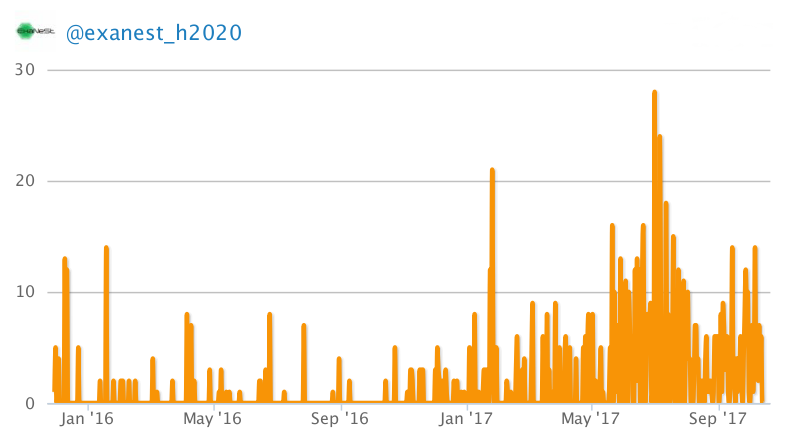
\includegraphics[width=1\linewidth]{Images/Tweets_Exanest.png}
   \caption{} 
 \end{subfigure}

 \begin{subfigure}[t]{0.9\textwidth}
   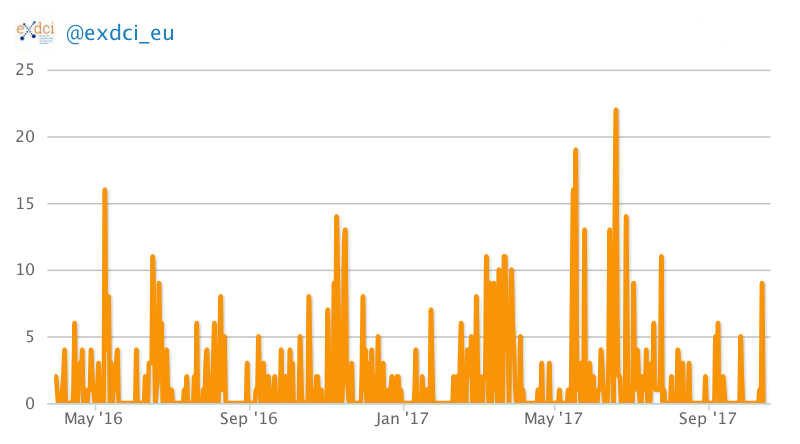
\includegraphics[width=1\linewidth]{Images/Tweets_Exdci.png}
   \caption{}
 \end{subfigure}
 \caption{(a) Time distribution of the number of tweets with hashtag \#quantumcomputing posted between 7th and 14th October 2017. (b) As for (a) but over the time period between 20th and 25th October 2017.} 
 \label{Tweets_Exanest-Exdci}
\end{figure}

\begin{figure}
 \centering
 \begin{subfigure}[t]{0.9\textwidth}
   \includegraphics[width=1\linewidth]{Images/Tweets_Montblanc.png}
   \caption{} 
 \end{subfigure}

 \begin{subfigure}[t]{0.9\textwidth}
   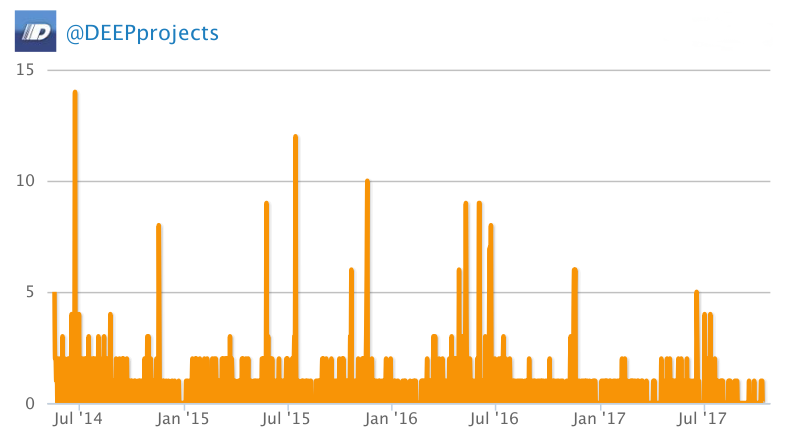
\includegraphics[width=1\linewidth]{Images/Tweets_Deepest.png}
   \caption{}
 \end{subfigure}
 \caption{(a) Time distribution of the number of tweets with hashtag \#quantumcomputing posted between 7th and 14th October 2017. (b) As for (a) but over the time period between 20th and 25th October 2017.} 
 \label{Tweets_Montblanc-Deepest}
\end{figure}

\section{Influence}
To find what are the HPC projects more influent on twitter, the data in table \ref{HPC_influence_table}. Data are updated to 14th October 2017. Influent projects on twitter are identified with the following conditions: high number of followers and high ratio followers/following. These data are were collected with twitonomy and are shown in table \ref{HPC_influence_table}.

The values in the table are shown in figure \ref{HPC_influence_plot}. The plot shows that the most influent HPC projects are identified by the conditions followers more than 100 and ratio larger than 2. These two values were identified by calculating the median of the number of followers and of the ratio followers/following of HPC projects. These projects are ExaFLOW, EXDCI, NEXTGenIO and READEX.

\begin{table}[t]
 \begin{center}
 {\scriptsize
  \begin{tabular}{cccc}
   \hline 
   \hline
   Project & Followers & Following & Followers/Following \\ 
   \hline
   \hline
   ALLScale & 41 & 28 & 1.46 \\
   ANTAREX & 77 & 13 & 5.92 \\
   COMPAT & 131 & 160 & 0.82 \\
   DEEP-EST & 697 & 534 & 1.31 \\
   ECOSCALE & 42 & 1 & 42 \\
   EuroLab-4-HPC 24 & 2 & 12 \\
   ExaFLOW & 206 & 90 & 2.29 \\
   ExaNeSt & 211 & 261 & 0.81  \\
   ExaNoDe & 52 & 54 & 0.96 \\
   EXDCI & 405 & 169 & 2.40 \\
   EXTRA & 45 & 18 & 2.50\\
   INTERTWINE & 106 & 59 & 1.80 \\
   MANGO & 74 & 46 & 1.61 \\
   Mont-Blanc 3 & 1 420 & 687 & 2.07 \\
   NEXTGenIO & 162 & 44 & 3.86 \\
   READEX & 116 & 55 & 2.11 \\
   SAGE & 122 & 86 & 1.42 \\ 
   FET & 6 499 & 1 612 & 4.03 \\
   \hline
   \hline
  \end{tabular}
 } 
 \end{center} 
 \caption{Summary of the Twitter analytics for the hashtag \#quantumcomputing over the monitored time periods. The potential reach is defined as the total aggregate number of followers of the people who mentioned the considered keyword in their tweets.}
\label{HPC_influence_table} 
\end{table}

\begin{figure}[!t] 
 \begin{center}
 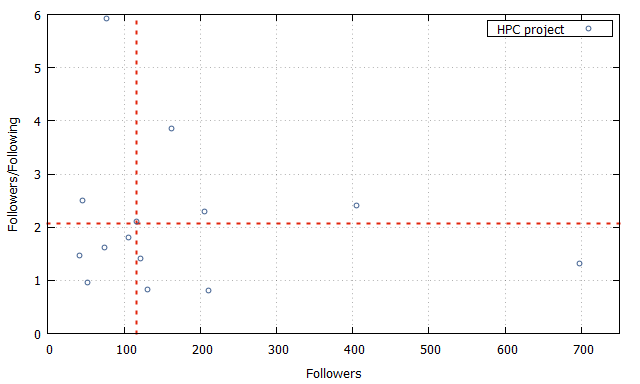
\includegraphics[scale=0.4]{Images/HPC_influence.png}
 \caption{Projects' distribution as a function of the available budget and of the number of considered online communication channels. The vertical lines are the budget medians of the group of projects with activated channels ranging between one and four. For the sake of clarity, the figure shows the budget range up to \euro 11.5 Million. The following projects were used for the medians calculation but lie outside the plotted budget range: QuantERA (\euro 40.5 Million, 3 channels), FLAG-ERA II (\euro 18.3 Million, two channels) and DEEP-EST (\euro 15.9 Million, 3 channels).}
 \label{HPC_influence_plot}
 \end{center}
\end{figure}

\section{Mentions of HPC projects}
A monitoring activity was launched to estimate the impact of HPC projects of Twitter. This was performed with the Twitter Analytics tool NUVI \cite{NUVI}. This activity monitored the mentions of the Twitter accounts of HPC projects from 1st July to 12th October 2017. The monitor activity analysed a total of 1323 social mentions. The time distribution of the mentions is shown in figure \ref{NUVI_time_distribution}.

The peak of conversation happened on 12th September 2017. It consisted of 59 mentions, with the most frequently used keywords during that peak being filippo mantovani, workshop, server cpu, prototype and processors.

Out of the 1323 mentions, 637 were original mentions, which had the potential of reaching an audience of 172 720 users. This reach is calculated as the sum of the followers of the accounts mentioning the analysed keywords. Moreover, 116 unique profiles made a total of 686 reshares. Shares and re-tweets spread the mentions to an additional 233 974 people. The spread is calculated as the sum of the followers of the accounts which shared or retweeted the tweets with the mentions. Reach and spread together give an estimate of the potential audience which came across with the tweeted contents. Figure \ref{HPC_Most_reach_spread_popular} shows the mentions with the largest reach, spread and the most popular one. The ratio between reach and spread defines the viral coefficient, which is equal to 1.4, see figure \ref{HPC_viral_coefficient}. As the value of the viral coefficient is larger than one indicates that the mentions were extremely viral. 

\begin{figure}[!t] 
 \begin{center}
 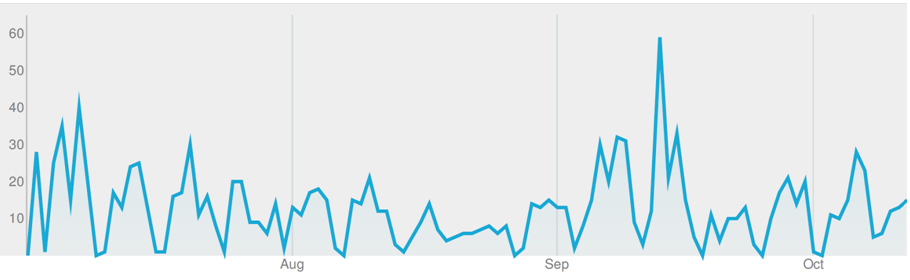
\includegraphics[scale=0.4]{Images/NUVI_time_distribution.png}
 \caption{Projects' distribution as a function of the available budget and of the number of considered online communication channels. The vertical lines are the budget medians of the group of projects with activated channels ranging between one and four. For the sake of clarity, the figure shows the budget range up to \euro 11.5 Million. The following projects were used for the medians calculation but lie outside the plotted budget range: QuantERA (\euro 40.5 Million, 3 channels), FLAG-ERA II (\euro 18.3 Million, two channels) and DEEP-EST (\euro 15.9 Million, 3 channels).}
 \label{NUVI_time_distribution}
 \end{center}
\end{figure}

\begin{figure}[!t] 
 \begin{center}
 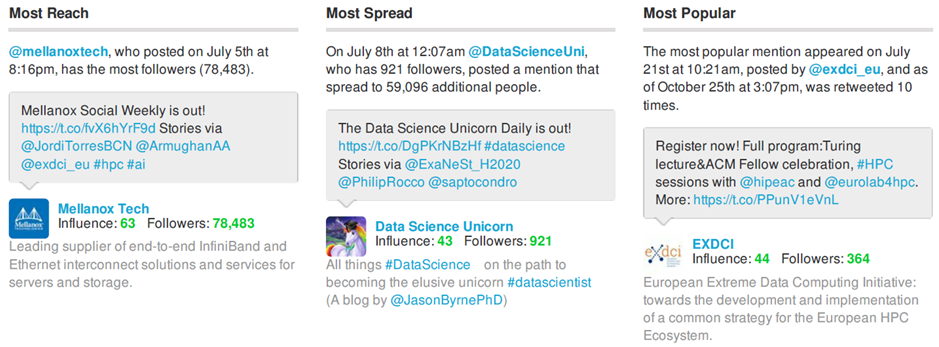
\includegraphics[scale=0.41]{Images/HPC_Most_reach_spread_popular.png}
 \caption{Projects' distribution as a function of the available budget and of the number of considered online communication channels. The vertical lines are the budget medians of the group of projects with activated channels ranging between one and four. For the sake of clarity, the figure shows the budget range up to \euro 11.5 Million. The following projects were used for the medians calculation but lie outside the plotted budget range: QuantERA (\euro 40.5 Million, 3 channels), FLAG-ERA II (\euro 18.3 Million, two channels) and DEEP-EST (\euro 15.9 Million, 3 channels).}
 \label{HPC_Most_reach_spread_popular}
 \end{center}
\end{figure}

\begin{figure}[!t] 
 \begin{center}
 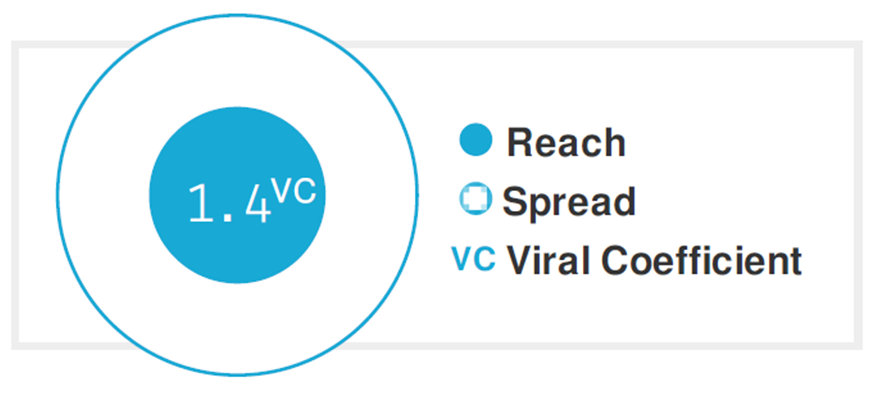
\includegraphics[scale=0.2]{Images/HPC_viral_coefficient.png}
 \caption{Projects' distribution as a function of the available budget and of the number of considered online communication channels. The vertical lines are the budget medians of the group of projects with activated channels ranging between one and four. For the sake of clarity, the figure shows the budget range up to \euro 11.5 Million. The following projects were used for the medians calculation but lie outside the plotted budget range: QuantERA (\euro 40.5 Million, 3 channels), FLAG-ERA II (\euro 18.3 Million, two channels) and DEEP-EST (\euro 15.9 Million, 3 channels).}
 \label{HPC_viral_coefficient}
 \end{center}
\end{figure}

An overview of the topics treated in the monitored mentions is provided in figure \ref{HPC_word_burst}. The figure is based on the 1005 mentions which came across 485 major categories over the monitored time. The list of most shared words is in table \ref{Most_shared_words}. 

\begin{figure}[!t] 
 \begin{center}
 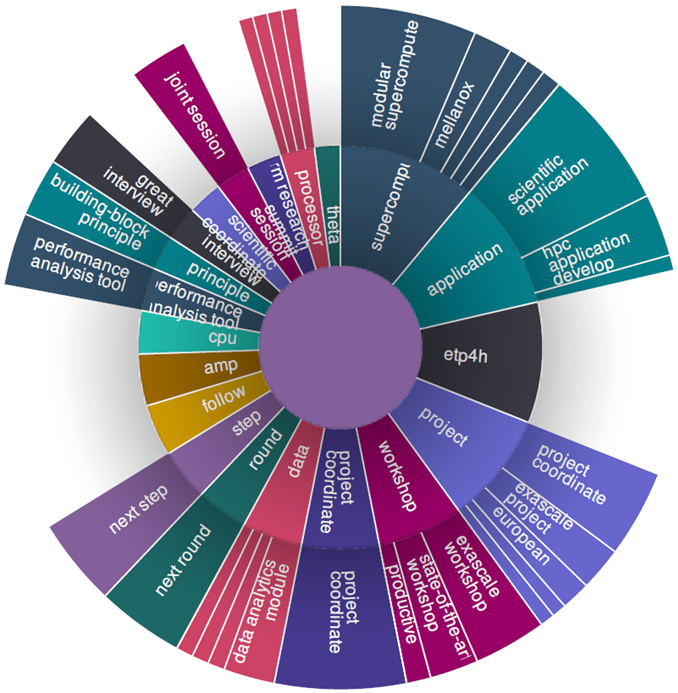
\includegraphics[scale=0.55]{Images/HPC_word_burst.png}
 \caption{Projects' distribution as a function of the available budget and of the number of considered online communication channels. The vertical lines are the budget medians of the group of projects with activated channels ranging between one and four. For the sake of clarity, the figure shows the budget range up to \euro 11.5 Million. The following projects were used for the medians calculation but lie outside the plotted budget range: QuantERA (\euro 40.5 Million, 3 channels), FLAG-ERA II (\euro 18.3 Million, two channels) and DEEP-EST (\euro 15.9 Million, 3 channels).}
 \label{HPC_word_burst}
 \end{center}
\end{figure}

\begin{table}[t]
 \begin{center}
 {\scriptsize
  \begin{tabular}{cccc}
   \hline 
   \hline
   Shared word & Mentions & Fraction of total mentions \\ 
   \hline
   \hline
   amp & 22 & 2.2\% \\
   project & 18 & 1.8\% \\
   supercomputer & 16 & 1.6\% \\
   application & 15 & 1.5\% \\
   etp4h & 14 & 1.4\% \\
   compute & 11 & 1.1\% \\
   \hline
   \hline
  \end{tabular}
 } 
 \end{center} 
 \caption{Summary of the Twitter analytics for the hashtag \#quantumcomputing over the monitored time periods. The potential reach is defined as the total aggregate number of followers of the people who mentioned the considered keyword in their tweets.}
\label{Most_shared_words} 
\end{table}